\RequirePackage{plautopatch}

\documentclass[gutter=20mm,fore-edge=20mm,head_space=30mm,foot_space=30mm]{jlreq}

% 数式
\usepackage{amsmath,amsfonts,amssymb}
\usepackage{bm}
% 画像
\usepackage[dvipdfmx]{graphicx}

\usepackage{url}
\usepackage[english]{babel}
\usepackage{wrapfig}
\usepackage{float}

\usepackage{siunitx}
\usepackage{enumerate}
\usepackage{enumitem}
\usepackage{multirow}
\usepackage{caption}
\usepackage{listings,jvlisting} %日本語のコメントアウトをする場合jvlisting(もしくはjlisting)が必要
%ここからソースコードの表示に関する設定
\lstset{
  basicstyle={\ttfamily},
  identifierstyle={\small},
  commentstyle={\smallitshape},
  keywordstyle={\small\bfseries},
  ndkeywordstyle={\small},
  stringstyle={\small\ttfamily},
  frame={tb},
  breaklines=true,
  columns=[l]{fullflexible},
  numbers=left,
  xrightmargin=0zw,
  xleftmargin=3zw,
  numberstyle={\scriptsize},
  stepnumber=1,
  numbersep=1zw,
  lineskip=-0.5ex
}

\usepackage{mathtools}
\usepackage{empheq}


\makeatletter
\newcommand{\figcaption}[1]{\def\@captype{figure}\caption{#1}}
\newcommand{\tblcaption}[1]{\def\@captype{table}\caption{#1}}
\makeatother
\pagestyle{plain}

\title{数値解析レポートNo.4}
\author{4年39番 湯嶋 皓騎}
\date{\number\year{}年\number\month{}月\number\day{}日}

\begin{document}
\newcommand*{\mathun}[1]{{\,\mathrm{[#1]}}}
\newcommand*{\textun}[1]{$\mathun{#1}$}
\renewcommand{\figurename}{Fig. }
\renewcommand{\lstlistingname}{List.}
\renewcommand{\refname}{参考文献}
\maketitle

\section{連立微分方程式}
\subsection{問題}
以下を満たす $(x, y)$ を $t = [0,2]$ の範囲で求めよ.

\begin{empheq}[left={\empheqlbrace}]{alignat=2}
  & \frac{dx}{dt} = x + 6y + t - 10 ,\ \ & x(0) = 1 \label{eq:dxdt} \\ %chktex 8 chktex 26 chktex 36
  & \frac{dy}{dt} = x + t - 3 ,& y(0) = 2 \label{eq:dydt} %chktex 8 chktex 26 chktex 36
\end{empheq}
\subsection{解法の検討}
式\ref{eq:dxdt} を $f(x, y; t)$, 式\ref{eq:dydt} を $g(x, y; t)$ とおくと,
\begin{empheq}[left={\empheqlbrace}]{alignat=2}
  x =& x(0) + \int_{t_0}^{t} f(x, y; t)dt \label{eq:xdt} \\ %chktex 8 chktex 26 chktex 36
  y =& y(0) + \int_{t_0}^{t} g(x, y; t)dt \label{eq:ydt}  %chktex 8 chktex 26 chktex 36
\end{empheq}
と表わされる.第二項の定積分を数値的に求めることで,$x, y$ を求めることができる.

\subsubsection{オイラー法を用いた解法}
ここで $x, y$ を定数 $(x_i, y_i)$ として $t = t_i$ $(i=0,1,2,\ldots)$ で一次のテイラー展開をすると,
\begin{empheq}[left={\empheqlbrace}]{alignat=2}
  x_{i+1} =& x_i + f(x_i, y_i; t_i)\Delta{} t \label{eq:x0} \\ %chktex 8 chktex 26 chktex 36
  y_{i+1} =& y_i + g(x_i, y_i; t_i)\Delta{} t \label{eq:y0} %chktex 8 chktex 26 chktex 36
\end{empheq}

とできる.これを用いて $t = 0$ から $t = 2$ までの範囲で $x, y$ を求める.実装の主要部をList.\ref{src:sod.c}に示す.
\begin{lstlisting}[caption=sod.c,label=src:sod.c]
#define PARAM_FILENAME "sod.csv"
#define UNUSED(x) (void)(x)

typedef double (*F)(double, double, double);
typedef struct {
    F f;
    F g;
    double x0;
    double y0;
    double width;
    double t0;
    double t_inf;
} Condition;

double f(double x, double y, double t) { return x + 6 * y + t - 10; }
double g(double x, double y, double t) {
    UNUSED(y);
    return x + t - 3;
}

Matrix *solve_sod(Condition *cond) {
    size_t len =
        (size_t)((cond->t_inf - cond->t0) / cond->width) + 1;  // len = n + 1
    Matrix *matrix = allocMatrix(3, len);  // data[0][i] = x_i, data[1][i] = y_i, data[2][i] = t_i
    size_t i;
    double *x = matrix->data[0];
    double *y = matrix->data[1];
    double *t = matrix->data[2];

    if (matrix == NULL) {
        fprintf(stderr, "Error: allocMatrix() failed.\n");
        return NULL;
    }

    x[0] = cond->x0;
    y[0] = cond->y0;
    t[0] = cond->t0;
    for (i = 1; i < len; i++) {
        x[i] = x[i - 1] + cond->f(x[i - 1], y[i - 1], t[i - 1]) * cond->width;
        y[i] = y[i - 1] + cond->g(x[i - 1], y[i - 1], t[i - 1]) * cond->width;
        t[i] = cond->t0 + cond->width * i;
    }

    return matrix;
}
\end{lstlisting}

ここで,\verb|UNUSED| マクロは引数を使わないことを明示するためのマクロであり,これによりコンパイラの警告を抑制している.また,連立常微分方程式の解を求める関数 \verb|solve_sod| は,\verb|Condition| 構造体を引数に取り,その構造体には$\displaystyle \frac{dx}{dt}, \frac{dy}{dt}$を表わす関数 \verb|f|, \verb|g|, 初期値 \verb|x0, y0|, 刻み幅 \verb|width|, 時刻の初期値 \verb|t0|, 時刻の終端値 \verb|t_inf| が含まれている.


\subsubsection{ルンゲ・クッタ法を用いた解法}
ルンゲ・クッタ法を用いて連立微分方程式を解くこともできる.ルンゲ・クッタ法はオイラー法を改良したものであり,4次のルンゲ・クッタ法は $O(h^5)$ の精度を持つ.
実装をList.\ref{src:rk.c}に示す.
\begin{lstlisting}[caption=rk.c,label=src:rk.c]
Matrix *solve_sod1(Condition *cond) {
    size_t len =
        (size_t)((cond->t_inf - cond->t0) / cond->width) + 1;  // len = n + 1
    Matrix *matrix = allocMatrix(3, len);  // data[0][i] = x_i, data[1][i] = y_i
    size_t i;
    double *x = matrix->data[0];
    double *y = matrix->data[1];
    double *t = matrix->data[2];

    if (matrix == NULL) {
        fprintf(stderr, "Error: allocMatrix() failed.\n");
        return NULL;
    }

    x[0] = cond->x0;
    y[0] = cond->y0;
    for (i = 1; i < len; i++) {
        double kx[4], ky[4];
        kx[0] = cond->f(x[i - 1], y[i - 1], t[i - 1]);
        ky[0] = cond->g(x[i - 1], y[i - 1], t[i - 1]);
        kx[1] = cond->f(x[i - 1] + cond->width / 2 * kx[0],
                        y[i - 1] + cond->width / 2 * ky[0],
                        t[i - 1] + cond->width / 2);
        ky[1] = cond->g(x[i - 1] + cond->width / 2 * kx[0],
                        y[i - 1] + cond->width / 2 * ky[0],
                        t[i - 1] + cond->width / 2);
        kx[2] = cond->f(x[i - 1] + cond->width / 2 * kx[1],
                        y[i - 1] + cond->width / 2 * ky[1],
                        t[i - 1] + cond->width / 2);
        ky[2] = cond->g(x[i - 1] + cond->width / 2 * kx[1],
                        y[i - 1] + cond->width / 2 * ky[1],
                        t[i - 1] + cond->width / 2);
        kx[3] = cond->f(x[i - 1] + cond->width * kx[2],
                        y[i - 1] + cond->width * ky[2], t[i - 1] + cond->width);
        ky[3] = cond->g(x[i - 1] + cond->width * kx[2],
                        y[i - 1] + cond->width * ky[2], t[i - 1] + cond->width);

        x[i] = x[i - 1] +
               cond->width * (kx[0] + 2 * kx[1] + 2 * kx[2] + kx[3]) / 6;
        y[i] = y[i - 1] +
               cond->width * (ky[0] + 2 * ky[1] + 2 * ky[2] + ky[3]) / 6;
        t[i] = t[i - 1] + cond->width;
    }

    return matrix;
}
\end{lstlisting}

1変数関数の数値積分とは異なり,$x$と$y$両方の仮ステップ$k$を求める必要があるため,\verb|kx|, \verb|ky|を配列として定義している.また,ルンゲ・クッタ法は4次のルンゲ・クッタ法を用いている.

\subsection{実行結果}
式~\ref{eq:xdt},~\ref{eq:ydt}を満たす$(x,y)$を$t=[0,2]$の範囲で求めるために,List.~\ref{src:sodin.csv}を入力に与えた.
\begin{lstlisting}[caption=sodin.csv,label=src:sodin.csv]
1,2,0.1,0,2
\end{lstlisting}
List.~\ref{src:sodin.csv}は初期値$x(0) = 1, y(0) = 2$に対して$t=0$から$t=2$までステップ幅$0.1$で求めることを指示している.
プログラムの出力は$x,y,t$の順で出力される.
\subsubsection{オイラー法}
List.~\ref{src:sod.c}を実行した結果をList.~\ref{src:sod.csv}に示す.
\lstinputlisting[caption=eular.csv,label=src:sod.csv]{1-1-20.csv} %chktex 8

List.~\ref{src:sod.csv}に加えてステップ幅を$0.2, 0.5$に設定したものと解析解を重ねて描画したものをFig.\ref{fig:sod}に示す.解析解の曲線描画にはgnuplotの\verb|set parametric|オプションを用いた.
\begin{figure}[H]
  \centering
  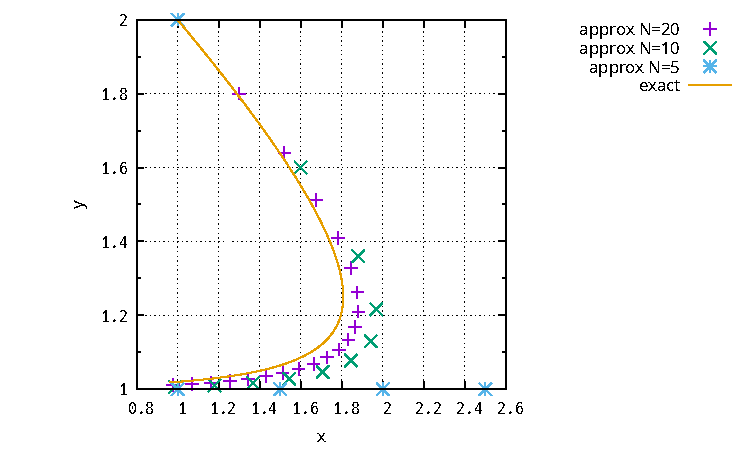
\includegraphics[width=0.8\linewidth]{1-1.pdf} %chktex 8
  \caption{オイラー法を用いた連立微分方程式の解}
  \label{fig:sod}
\end{figure}

まずは Fig.\ref{fig:sod}の分割数$N=20$の点群と解析解を比較する.この連立微分方程式は初期値 $(x_0, y_0) = (1, 2)$ を与えたとき,$(x, y) = (1.8, 1.25)$ 付近までは$x$が増加し$y$が減少しているが,
それ以降は$x$も$y$も減少していることがわかる.また,ステップ幅を$0.1$としたとき,解析解との最大誤差は $0.1$ 程度であった.数値解と解析解の誤差はグラフの変化が激しい部分で大きくなっている.これは式~\ref{eq:x0},~\ref{eq:y0}で一次のテイラー展開を用いているためである.

次に,ステップ幅を変化させたときの数値解と解析解の乖離を確認する.ステップ幅が$0.1, 0.2$のときは解析解の形状に近いが,ステップ幅が$0.5$のときは大きく乖離している.List.~\ref{src:115.csv}にステップ幅$0.5$の実行結果を示す.
\lstinputlisting[caption=1-1-5.csv,label=src:115.csv]{1-1-5.csv} %chktex 8
これはステップ幅を$0.5$に設定したとき,$g(x_i, y_i; t_i)$が$t_0$以外で$0$になってしまうためである.これより,オイラー法ではステップ幅が大きいときには誤差が非常に大きくなる場合があることがわかる.

\subsubsection{ルンゲ・クッタ法}
ステップ幅を$0.5$としたときの実行結果をList.~\ref{src:sod1.csv}に示す.
\lstinputlisting[caption=rk.csv,label=src:sod1.csv]{1-2-5.csv} %chktex 8
List.~\ref{src:sod1.csv}と解析解を重ねて描画したものをFig.\ref{fig:sod1}に示す.ステップ幅は$0.1, 0.2, 0.5$の3通りで実行し,図中には分割数 $N$ で示している.
\begin{figure}[H]
  \centering
  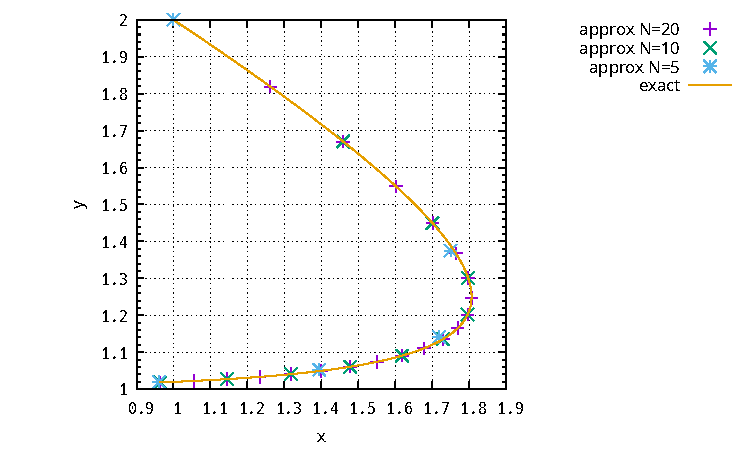
\includegraphics[width=0.8\linewidth]{1-2.pdf} %chktex 8
  \caption{ルンゲ・クッタ法を用いた連立微分方程式の解}
  \label{fig:sod1}
\end{figure}
いずれのステップ幅においても,オイラー法より誤差が小さくほとんど解析解と一致していることがわかる.

\section{高次微分方程式}
\subsection{問題}
式\ref{eq:2nd}の$x=1$における微分方程式の解$y$を求めよ.
\begin{equation}
  \frac{d^2y}{dx^2} + 5\frac{dy}{dx} - 6y = 0 \label{eq:2nd}
\end{equation}
ここで,初期条件は$\displaystyle y(0) = 0, \frac{dy}{dx}(0) = 7$とする.

\subsection{解法の検討}
$\displaystyle \frac{dy}{dx} = z$とおくと,式\ref{eq:2nd}は式\ref{eq:2nd2}のように表わされる.
\begin{align}
  \frac{dz}{dx} + 5z - 6y & = 0 \nonumber             \\
  \frac{dz}{dx}           & = 6y - 5z \label{eq:2nd2}
\end{align}

これらは独立変数 $x$ に関する連立常微分方程式であるから,先の問題と同様に解くことができる.

$f(y, z; x) = z, g(y, z; x) = 6y - 5z$とおき,$x = 0$での初期条件$\displaystyle y(0) = 0, z(0) = 7$に対してルンゲ・クッタ法を用いて解く.List.~\ref{src:rk.c}で示したプログラムは独立変数$t$に関する$x, y$の連立微分方程式を解くものであるため,$y \rightarrow x, z \rightarrow y, x \rightarrow t$と変数変換して用いることとする.

\subsection{実装}

プログラムをList.\ref{src:2nd.c}に示す.ここで\verb|solve_sod1()|はルンゲ・クッタ法を用いて連立微分方程式を解く関数である.
\begin{lstlisting}[caption=2nd.c,label=src:2nd.c]
double f(double y, double z, double x) {
    UNUSED(y);
    UNUSED(x);
    return z;
}
double g(double y, double z, double x) {
    UNUSED(x);
    return 6 * y - 5 * z;
}

int main(void) {
    Matrix *matrix, *res;
    size_t i;
    Condition cond;

    // データの読み込みと検証

    cond = (Condition){
        .f = f,
        .g = g,
        .x0 = matrix->data[0][0],
        .y0 = matrix->data[0][1],
        .width = matrix->data[0][2],
        .t0 = matrix->data[0][3],
        .t_inf = matrix->data[0][4],
    };
    printf("#step width: %f\n", cond.width);
    res = solve_sod1(&cond);
    if (res == NULL) {
        freeMatrix(matrix);
        return EXIT_FAILURE;
    }

    for (i = 0; i < res->col; i++) {
        printf("%.6f,%.6f,%.6f\n", res->data[0][i], res->data[1][i],
               res->data[2][i]);
    }

    freeMatrix(res);
    freeMatrix(matrix);

    return EXIT_SUCCESS;
}
\end{lstlisting}
このプログラムを実行すると,1列目に$y$,2列目に$z$,3列目に$x$が出力される.

\subsubsection{実行結果}
$x=1$での$y$の値を求めるために,List.~\ref{src:2ndin.csv}を入力に与えた.
\begin{lstlisting}[caption=2ndin.csv,label=src:2ndin.csv]
0,7,0.1,0,1
\end{lstlisting}
List.~\ref{src:2ndin.csv}は初期値$y(0) = 0, z(0) = 7$に対して$x=0$から$x=1$までステップ幅$0.1$で求めることを指示している.
実行した結果をList.~\ref{src:2nd.csv}に示す.

\begin{lstlisting}[caption=2nd.csv,label=src:2nd.csv]
#step width: 0.100000
0.000000,7.000000,0.000000
0.555771,4.401571,0.100000
0.919562,3.032445,0.200000
1.184027,2.344845,0.300000
1.400717,2.038470,0.400000
1.598666,1.949048,0.500000
1.794618,1.987118,0.600000
1.998643,2.104402,0.700000
2.217239,2.275343,0.800000
2.455041,2.486963,0.900000
2.715774,2.733312,1.000000
\end{lstlisting}

csvファイルの1列目と3列目より,$x=1$における$y$の値は$2.715774$であることがわかる.
解析解$y = e^x - e^{-6x}$に $x=1$ を代入した結果は$2.715803$であるため,相対誤差は
\begin{equation}
  \frac{|2.715774 - 2.715803|}{2.715803} \times 100 = 0.0011\mathun{\%}
\end{equation}
であり,非常に高い精度で数値解が解析解と一致していることがわかる.

次に,List.~\ref{src:2nd.csv}を解析解と重ねてプロットした結果をFig.~\ref{fig:2nd}に示す.
今回は$x=1$での解が正しく求められればよいため,ステップ幅は変化させず$0.1$のみ実行した.
\begin{figure}[H]
  \centering
  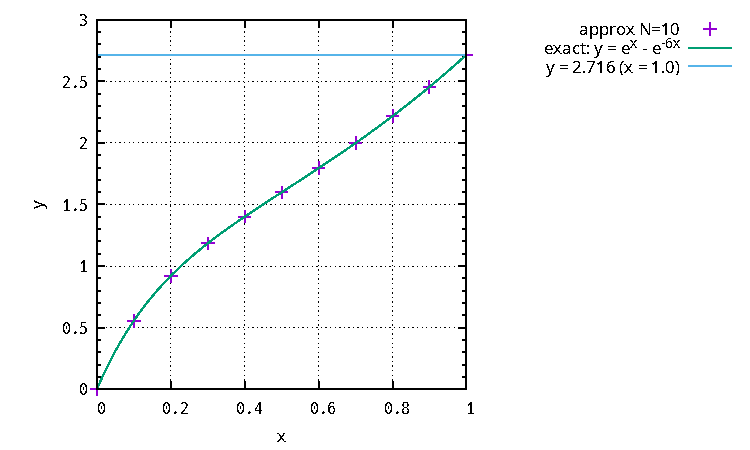
\includegraphics[width=0.8\linewidth]{2-10.pdf} %chktex 8
  \caption{高次微分方程式の解}
  \label{fig:2nd}
\end{figure}

Fig.~\ref{fig:2nd}より,解析解と数値解は広い範囲において高い精度で一致していることがわかる.

\section{感想}
ルンゲ・クッタ法はオイラー法と比べて高い精度を持つことを改めて確認できた.数値解析で学んだことを卒業研究でも活かしていきたい.

\begin{thebibliography}{99}
  \bibitem{} gnuplotでグラフに文字を書く -- 米澤進吾 ホームページ \url{https://sk.kuee.kyoto-u.ac.jp/person/yonezawa/contents/program/gnuplot/label.html} %chktex 8
\end{thebibliography}

\end{document}
